% !TeX spellcheck = de_CH_frami

\section{Laplace Operator und Graphen\label{sec:sgwt:laplace}}
\rhead{Laplace Operator und Graphen}

F\"ur die Analyse und Synthese von Funktionen auf Graphen und deren Spektren 
spielen der Laplace Operator und besonders die Laplace Matrix eine wichtige 
Rolle. Analog den Graphen in~\cref{sec:sgwt:graphs}, wollen wir zuerst 
auf die Grundlagen des Laplace Operators in~\cref{subsec:sgwt:laplaceop} und 
der Laplace Matrix \laplaceL{} in~\cref{subsec:sgwt:laplacem} eingehen. 
In~\cref{sec:sgwt:spectralanalysis} folgt dann die Analyse des Spektrums und 
Konstruktion der SGWT.

\subsection{Laplace Operator\label{subsec:sgwt:laplaceop}}
\rhead{Laplace Operator}

Der Laplace Operator $\Delta$ in $\mathbb{R}^n$ wird im kartesischen 
Koordinatensystem durch die Summe der $n$~zweiten Ableitungen
\begin{equation*}
\Delta = 
\sum_{i = 1}^{n}\frac{\partial^2}{\partial x_i^2}
=
\frac{\partial^2}{\partial x_1^2}
+ \frac{\partial^2}{\partial x_2^2}
+ \dots
+ \frac{\partial^2}{\partial x_n^2}
\end{equation*}
beschrieben. H\"aufig trifft man erstmals auf den Laplace Operator wenn man 
versucht die Poisson-Gleichung $-\Delta u = f$ zu l\"osen.

Wie Anfangs bereits beschrieben, sind unsere Daten meist nur in diskreter Form 
vorhanden. Daher w\"are es vorteilhaft, auch eine diskretisierte oder zumindest 
approximierte Form des Laplace Operators zu haben.

\subsection{Finite-Differenzen}
\rhead{Finite-Differenzen}

Finite-Differenzen erlauben uns eine diskrete Approximation des 
Laplace Operators. Sie erm\"oglichen uns also genau das, was wir 
in~\cref{subsec:sgwt:laplaceop} gesucht haben.

Als Ausgangslage nehmen wir die Funktion $u(x)$ mit dem eindimensionalen 
Definitionsbereich $u: \mathbb{R} \rightarrow \mathbb{R}$ und beginnen zuerst 
mit der Approximation der ersten Ableitung an der Stelle $x_i$, mit dem Abstand 
$h = \Delta x_i$,
\begin{equation*}
\frac{\partial u}{\partial x_i}
= \frac{u(x_i+h)-u(x_i)}{h}.
\end{equation*}
Indem wir diese Gleichung nochmals ableiten, erhalten wir die f\"ur den Laplace 
Operator relevante zweite Ableitung
\begin{equation*}
\frac{\partial}{\partial x_i}\frac{\partial}{\partial x_i}u
= \frac{\partial^2 u}{\partial x_i^2}
= \frac{\frac{u(x_i+h)-u(x_i)}{h}-\frac{u(x_i)-u(x_i+h)}{h}}{h}
= \frac{u(x_i+h)-2u(x_i)+u(x_i-h)}{h^2}.
\end{equation*}

Dies k\"onnen wir nat\"urlich auch in zwei Dimensionen mit Funktionen der Art 
$u(x, y)$ machen. Wieder wenden wir zuerst den Laplace Operator $\Delta$ auf 
unser $u$ an und erhalten
\begin{equation*}
\Delta u(x, y) = u_{xx}(x, y) + u_{yy}(x, y).
\end{equation*}
Dies k\"onnen wir wiederum mittels Finiten-Differenzen approximieren, mit $h = 
\Delta x = \Delta y$ liefert uns das
\begin{align}
\Delta u(x,y)
&=
\frac{u(x+h,y)-2u(x, y)+u(x-h,y)}{h^2}
+\frac{u(x,y+h)-2u(x, y)+u(x,y-h)}{h^2} \nonumber \\
&=
\frac{u(x+h,y)+u(x-h,y)+u(x,y+h)+u(x,y-h)-4u(x, y)}{h^2}.
\label{eq:sgwt:fivepointstencil}
\end{align}
Dieser Operator ist auch bekannt als der F\"unfpunkte-Stern-Operator 
oder five-point stencil (im Englischen), siehe~\cref{fig:sgwt:graph:star}.
\begin{figure}
\centering
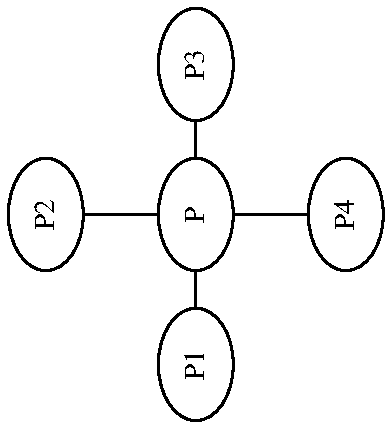
\includegraphics[
angle=-90,
origin=c,
scale=0.6
]{papers/sgwt/images/star.pdf}
\vspace{0pt}
\caption{F\"unfpunkte-Stern-Operator mit $P = u(x,y), P_1 = 
u(x-h,y), P_2 = u(x,y+h), P_3 = u(x+h,y), P_4 = u(x,y-h)$.
\label{fig:sgwt:graph:star}}
\end{figure}

Es folgt daraus, dass bei der zweiten Ableitung die ``aufeinanderfolgenden 
Differenzen'' immer den Knoten in der Mitte gemeinsam haben. Damit k\"onnen 
wir nun wieder zur\"uck auf unsere Graphen 
in~\cref{fig:sgwt:graph:simple} aus~\cref{sec:sgwt:graphs} kommen. Wenn wir 
diesen n\"amlich mit dem den F\"unfpunkte-Stern-Operator 
aus~\cref{fig:sgwt:graph:star} vergleichen, wird klar, dass der Graph, obwohl 
er auf den ersten Blick anders aussieht, der Gleiche ist. Wenn wir also den 
Laplace Operator auf den jeweiligen Graph anwenden, werden wir das gleiche 
Resultat erhalten.

Wir k\"onnen somit noch einen Schritt weitergehen und uns von den Achsen 
l\"osen. Nehmen wir als Beispiel den Graphen aus~\cref{fig:sgwt:laplace:nstar}. 
F\"ur die zweite Ableitung beim Punkt P brauchen wir also nach dem Schema 
aus~\cref{eq:sgwt:fivepointstencil} die Summe aller Funktionswerte $u(P_1)$ bis 
$u(P_8)$ abz\"uglich Anzahl Nachbarn von $P$, also dem Grad $d(P)$, 
multipliziert mit dem Funktionswert $u(P)$, was uns folgende Gleichung
\begin{equation*}
\Delta u = \frac{1}{h^2}\left(\sum_{i = 1}^{8}u(P_i) - 8u(P)\right)
\end{equation*}
liefert. Generell erhalten wir f\"ur den Laplace Operator an einem Knoten $v$ 
mit $n$~Nachbarn die Definition
\begin{equation}
\Delta u = \frac{1}{h^2}\left(\sum_{i = 1}^{n}u(v_i) - d(v)u(v)\right).
\label{eq:sgwt:generallaplace}
\end{equation}

\begin{figure}
\centering
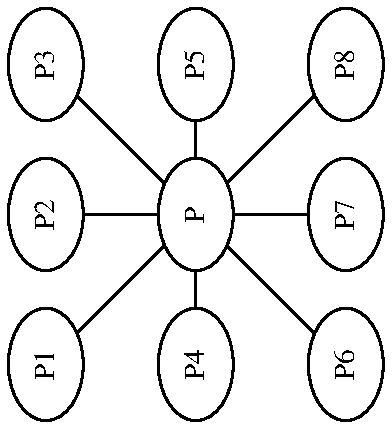
\includegraphics[
angle=-90,
origin=c,
scale=0.7
]{papers/sgwt/images/nstar.pdf}
\vspace{0pt}
\caption{Ein Graph mit neun Knoten und acht Kanten. Der Knote P mit Grad 
$d(P) = 8$ sticht hier klar gegen\"uber den anderen Knoten mit jeweils 
Grad $d(\text{P}_i) = 1$ hervor.
    \label{fig:sgwt:laplace:nstar}}
\end{figure}

\subsection{Laplace Matrix\label{subsec:sgwt:laplacem}}
\rhead{Laplace Matrix}

Wenn wir nun mit Hilfe von Taschenrechnern oder Computer rechnen wollen, ist 
meist die Darstellung in Form einer Matrix besonders geeignet. Die Laplace 
Matrix \laplaceL{}~\cite{noauthor_laplace-matrix_2017} ist genau 
dies. Sie basiert auf der Nachbarschaft der einzelnen Knoten und deren Grad, 
welche in der Adjazenzmatrix und der Gradmatrix codiert werden k\"onnen.

\subsubsection{Adjazenzmatrix \texorpdfstring{\adjacencyM{}}{A}}

Die Adjazenzmatrix \adjacencyM{}~\cite{noauthor_adjacency_2019} codiert die 
Nachbarschaftsbeziehungen innerhalb eines Graphen. Ihre Zeilen und Spalten 
stehen dabei f\"ur die einzelnen Knoten und die Werte der Matrix f\"ur das 
Gewicht der einzelnen Kanten zwischen den jeweiligen Knoten. Da wir keine 
Verbindung von einem Knoten zu sich selber zulassen, wird die Diagonale immer 
$0$ sein. 

Als Beispiele nehmen wir den Graphen aus~\cref{fig:sgwt:graph:simple} und den 
gewichteten Graphen aus~\cref{fig:sgwt:graph:simpleweight}. F\"ur ersteren 
erhalten wir die Adjazenzmatrix
\begin{equation*}
\adjacencyM =
\begin{bmatrix}
0 & 1 & 0 & 0 & 0 \\
1 & 0 & 1 & 1 & 1 \\
0 & 1 & 0 & 0 & 0 \\
0 & 1 & 0 & 0 & 0 \\
0 & 1 & 0 & 0 & 0
\end{bmatrix}
\end{equation*}
und f\"ur letzteren
\begin{equation*}
\adjacencyM =
\begin{bmatrix}
0 & 1 & 0 & 0 & 0 \\
1 & 0 & 1.2 & 0.4 & 0.8 \\
0 & 1.2 & 0 & 0 & 0 \\
0 & 0.4 & 0 & 0 & 0 \\
0 & 0.8 & 0 & 0 & 0
\end{bmatrix}.
\end{equation*}

\subsubsection{Gradmatrix \texorpdfstring{\degreeM{}}{D}}

Die Gradmatrix \degreeM{}~\cite{noauthor_degree_2018} codiert den Grad der 
einzelnen Knoten eines Graphen. Die Zielen und Spalten repr\"asentieren dabei, 
wie schon bei der Adjazenzmatrix \adjacencyM{}, die Knoten des Graphen. Damit 
ist klar, dass wir es hier mit einer Diagonalmatrix zu tun haben.

Auch hier nehmen wir wieder die Beispielgraphen 
aus~\cref{fig:sgwt:graph:simple} und~\cref{fig:sgwt:graph:simpleweight}. 
Ersterer hat die Gradmatrix
\begin{equation*}
\degreeM =
\begin{bmatrix}
1 & 0 & 0 & 0 & 0 \\
0 & 4 & 0 & 0 & 0 \\
0 & 0 & 1 & 0 & 0 \\
0 & 0 & 0 & 1 & 0 \\
0 & 0 & 0 & 0 & 1
\end{bmatrix}
\end{equation*}
und letzterer
\begin{equation*}
\degreeM =
\begin{bmatrix}
1 & 0 & 0 & 0 & 0 \\
0 & 3.4 & 0 & 0 & 0 \\
0 & 0 & 1.2 & 0 & 0 \\
0 & 0 & 0 & 0.4 & 0 \\
0 & 0 & 0 & 0 & 0.8
\end{bmatrix}.
\end{equation*}

\subsubsection{Laplace Matrix \texorpdfstring{\laplaceL{}}{L}}

Mit der Adjazenzmatrix und er Gradmatrix haben wir alles zusammen um die 
Laplace Matrix \laplaceL{} zu bestimmen. Diese setzt sich wie folgt zusammen
\begin{equation}
\laplaceL = \degreeM - \adjacencyM.
\label{eq:sgwt:laplace}
\end{equation}
Zur Veranschaulichung nehmen wir nochmals die Graphen 
aus~\cref{fig:sgwt:graph:simple} und~\cref{fig:sgwt:graph:simpleweight} und 
erhalten
\begin{equation*}
\laplaceL =
\begin{bmatrix}
1 & -1 & 0 & 0 & 0 \\
-1 & 4 & -1 & -1 & -1 \\
0 & -1 & 1 & 0 & 0 \\
0 & -1 & 0 & 1 & 0 \\
0 & -1 & 0 & 0 & 1
\end{bmatrix}
\end{equation*}
respektive
\begin{equation*}
\laplaceL =
\begin{bmatrix}
1 & -1 & 0 & 0 & 0 \\
-1 & 3.4 & -1.2 & -0.4 & -0.8 \\
0 & -1.2 & 1.2 & 0 & 0 \\
0 & -0.4 & 0 & 0.4 & 0 \\
0 & -0.8 & 0 & 0 & 0.8
\end{bmatrix}.
\end{equation*}

Im allgemeinen Fall eines gewichteten Graphen mit $n$ Knoten erhalten wir die 
Laplace Matrix
\begin{equation*}
\laplaceL =
\begin{bmatrix}
d_w(v_1) & -w(e_{v_1, v_2}) & \dotso & -w(e_{v_1, v_n}) \\
-w(e_{v_2, v_1}) & d_w(v_2) & \dotso & \vdots \\
\vdots & \vdots & \ddots &  \vdots \\
-w(e_{v_n, v_1}) & -w(e_{v_n, v_2}) & \dotso & d_w(v_n)
\end{bmatrix}.
\end{equation*}
Die Kantengewichtsfunktion $w(e)$ liefert dabei entweder das Kantengewicht 
falls $e \in E$ oder anderenfalls $0$. Im Fall des ungewichteten Graphen werden 
die Kanten jeweils alle mit $1$ gewichtet.

Aufgrund unserer Konstruktion von \laplaceL{} ist ersichtlich, dass die Summe 
der jeweiligen Zeilen und Spalten immer gleich $0$ sein wird. Womit wir bereits 
jetzt sagen k\"onnen, dass mindestens ein Eigenwert~$\lambda$ von \laplaceL{} 
auch gleich $0$ sein wird.

\subsubsection{Laplace Matrix \texorpdfstring{\laplaceL{}}{L} als 
Verallgemeinerung des Laplace-Operators \texorpdfstring{$\Delta$}{Delta}}

Wenn wir jetzt die Funktion $u$ auf die Laplace Matrix \laplaceL{} anwenden,
erhalten wir
\begin{align*}
\laplaceL u &=
\begin{bmatrix}
d_w(v_1) & -w(e_{v_1, v_2}) & \dotso & -w(e_{v_1, v_n}) \\
-w(e_{v_2, v_1}) & d_w(v_2) & \dotso & \vdots \\
\vdots & \vdots & \ddots &  \vdots \\
-w(e_{v_n, v_1}) & -w(e_{v_n, v_2}) & \dotso & d_w(v_n)
\end{bmatrix}
\begin{pmatrix}
u_0 \\
u_1 \\
\vdots \\
u_{N-1}
\end{pmatrix}\\
&=
\begin{pmatrix}
d_w(v_1)u_0 - w(e_{v_1, v_2}) u_1 - \dotsm -w(e_{v_1, v_N}) u_{n-1} \\
d_w(v_2)u_1 - w(e_{v_2, v_1}) u_0 - \dotsm -w(e_{v_2, v_N}) u_{n-1} \\
\vdots \\
d_w(v_n)u_{n-1} - w(e_{v_1, v_2}) u_0 - \dotsm -w(e_{v_N, v_{N-1}}) u_{n-2} \\
\end{pmatrix}\\
&=
d_w(v)u-\sum_{i\text{ Nachbarn}}^{n} w(e_i)u_i
.
\end{align*}
Wenn wir nun einen ungewichteten Graphen nehmen, der vollst\"andig verbunden 
ist, wo also jeder Knoten mit jedem anderen Verbunden ist, und dessen 
Kantengewichte alle gleich $\frac{1}{h^2}$ setzen, erhalten wir
\begin{equation*}
\laplaceL u =
\left(
    \frac{1}{h^2} n u - \sum_{i\text{ Nachbarn}}^{n} \frac{1}{h^2} u_i
\right)
=
-\frac{1}{h^2} n \left(
    \frac{1}{n}\sum_{i\text{ Nachbarn}}^{n} u_i - u
\right)
= -\Delta u.
\end{equation*}
Es zeigt sich also, dass die Laplace Matrix \laplaceL{} den bereits 
kennengelernten Laplace-Operator~$\Delta$ verallgemeinert, da wir damit nicht 
nur den vollst\"andig verbundenen, sondern auch jeden anderen Graphen abbilden 
k\"onnen.
